\chapter{Background}
The second chapter, \textit{Background}, explains the necessary background to fully understand the Bachelor thesis. 
In the first section, \textit{Definitions}, terms needed to understand the Bachelor thesis are defined.
In the second section, \textit{Methodology}, the used methodology is presented.
In the third section, \textit{Related Systems}, systems for iOS\footnote{iOS: \url{https://www.apple.com/ios/ios-13/}, (last accessed October 15, 2019)} are presented, that solve the problem of finding a parked car.
In the fourth section, \textit{Related Works}, academic works are discussed, that relate to the Bachelor thesis. It focuses on transportation mode classification.

\section{Definitions}

The first section, \textit{Definitions}, defines terms, that are not commonly known and necessary for understanding the Bachelor thesis. 

\paragraph{Spatial Trajectory} A spatial trajectory is a trace of an object through a geographical space. It is usually represented as a chronologically ordered list of points $ P = p_1\rightarrow p_2 \rightarrow \dots \rightarrow p_n$. The points consist of a geospatial coordinate set, and a timestamp $p_i=(lat,lon,t)$. \cite{Zheng:2015:TDM:2764959.2743025}

\paragraph{Semantic Trajectory} A semantic trajectory is defined as a finite spatial trajectory with a semantic meaning, i.e. the used transportation mode $((p_1\rightarrow p_2 \rightarrow \dots \rightarrow p_n), label)$. \cite{Zheng:2015:TDM:2764959.2743025}

\paragraph{Trajectory Segmentation} In trajectory segmentation, a trajectory is divided into fragments by a measure such as time, spatial shape, or semantic meaning. These fragments can be used for further processing such as classification. \cite{Zheng:2015:TDM:2764959.2743025}

\paragraph{Trajectory Classification} The process of predicting the class label of trajectories, or their segments, based on their features is called trajectory classification. \cite{lee2008traclass}

\paragraph{Stay Point} A stay point $s$ is defined as a geographical region in which a user stays over a threshold time $T_r$ within a threshold distance $D_r$. In a spatial trajectory, a stay point $s$ is characterised by a set of consecutive points $P=p_m \rightarrow p_{m+1} \rightarrow \dots \rightarrow p_n$ with $\forall m<i\leq n:\: Dist(p_m, p_i) \leq D_r$, $Dist(p_m, p_{n+1}) > D_r $, and $t(p_n) - t(p_m) \geq T_r$. The stay point $s$ is then defined by $s=(lat, lon, t_a, t_l)$ where $lat(s) = \sum^{n}_{i=m}lat(p_i) /|P|$, $lon(s) = \sum^{n}_{i=m}lon(p_i)/|P|$, $t_a(s) = t(p_m)$, and $t_l(s) = t(p_n)$. \cite{Zheng2007}

\paragraph{Segment} A segment is defined as the edge between any two consecutive points in a spatial trajectory. In a spatial trajectory $P=p_1 \rightarrow \dots \rightarrow p_n$, each edge $p_i\rightarrow p_{i+1}, 1\leq i < n$ is called a segment. \cite{Zheng:2015:TDM:2764959.2743025}

\paragraph{Trip} A trip $T_i$ is defined as the subset of a spatial trajectory between two consecutive stay points. $T_i = \{p \in P |\: s_i.t \leq p.t \leq s_{i+1}.t \}$, where $T_i$ is the set of all spatial trajectories of a trip, $P$ is the set off all recorded spatial trajectories of a user, and $s_i, s_{i+1}$ are two consecutive stay points of the user. \cite{Zheng2008}

\paragraph{Stage} A stage is a group of successive segments of the same transportation mode within a trip. A new stage starts where the transportation mode changes to another, or where the used vehicle is changed. \cite{Bolbol2012}

\paragraph{Change Point} A change point is defined as the location where a person changes their mode of transportation within a trip. \cite{Zheng2008}

\section{Methodology}
The second section, \textit{Methodology}, explains the methodology used for analyzing the problem, determining the users expectations of the application and ensuring the usability of the user interface of the application. It defines the way the requirements of the application are presented. The methodology is user-centric and similar to the User-Centered Design approach. 

A group of people is interviewed for background interviews. The goal of background interviews is to gain insight into the ''needs and expectations of users''. The interviews are performed with a semi-structured technique. In semi-structured interviews, the interviewer has a list of questions and the interviewee is encouraged to elaborate their answers. The interviewer can ask follow up questions if more insights in a specific answer are needed. This technique is used, because the detailed answers of the users allow insights into their expectations of the application and the option for asking follow up questions avoid imprecise answers. A structured technique would not allow the users to mention their own expectations and issues. A unstructured technique would make the answers of the interviewees difficult to compare. The answers given in the interviews are summarised. Based on the results of the interviews and the limitations of the Bachelor thesis, requirements for the application are defined. The requirements are separated into functional and non-functional requirements. \cite{Abras2004} \cite{wilson2013interview}

To ensure the usability of the application, the user interface is created iteratively. Best practises are applied by using design heuristics by Nielsen and conforming to the Human Design Guidelines by Apple Inc\footnote{Apple Inc: \url{https://www.apple.com/} (last accessed October 15, 2019)}. Iterative Design is defined as ''progressive refinement through cyclical data-driven development'' \cite{goodman2012observing}. During each iteration, users test the current design prototypes. For these tests, the think aloud method is used. Think aloud is ''a special kind of verbal protocol in which the user says out loud what she is thinking while she is carrying out a task or doing some problem solving'' \cite{nielsen1994usability}. The method is chosen, because it can lead to less design interactions while still resulting in efficient systems which are accepted by users. In the tests itself, a prototype of the user interface is provided to the user. The user is asked to perform different actions on the prototype and to think aloud. They are asked to elaborate what they are thinking and reasoning while using the prototype. After the tests are performed, the protocols of the tests are analysed for potential obstacles in the user interface. These obstacles in the user interface are removed in the next iteration. The tests are repeated with the new prototype to ensure the changes have actually a positive impact on the usability of the application. \cite{Abras2004} \cite{goodman2012observing} \cite{nielsen1994usability} \cite{heurisitcNielsen} \cite{apple:interfaceguidliines} \cite{jaspers2004think} 

The used methodology in the Bachelor thesis is user-centric. Semi-structured background interviews are performed to understand the needs and expectations of the users. Based on the results of the interviews, requirements for the application are defined. To ensure the usability of the user interface, the interface prototype is designed iteratively and following best practises. The iterations are evaluated with the think aloud method to find obstacles in the design. These obstacles are removed in the design of the following iteration. \cite{Abras2004} \cite{wilson2013interview} \cite{heurisitcNielsen} \cite{apple:interfaceguidliines}

\section{Related Systems}
The third section, \textit{Related Systems}, is a survey on existing systems for iOS, which determine the parking position of a users car.


\begin{figure}[h]
  \centering
  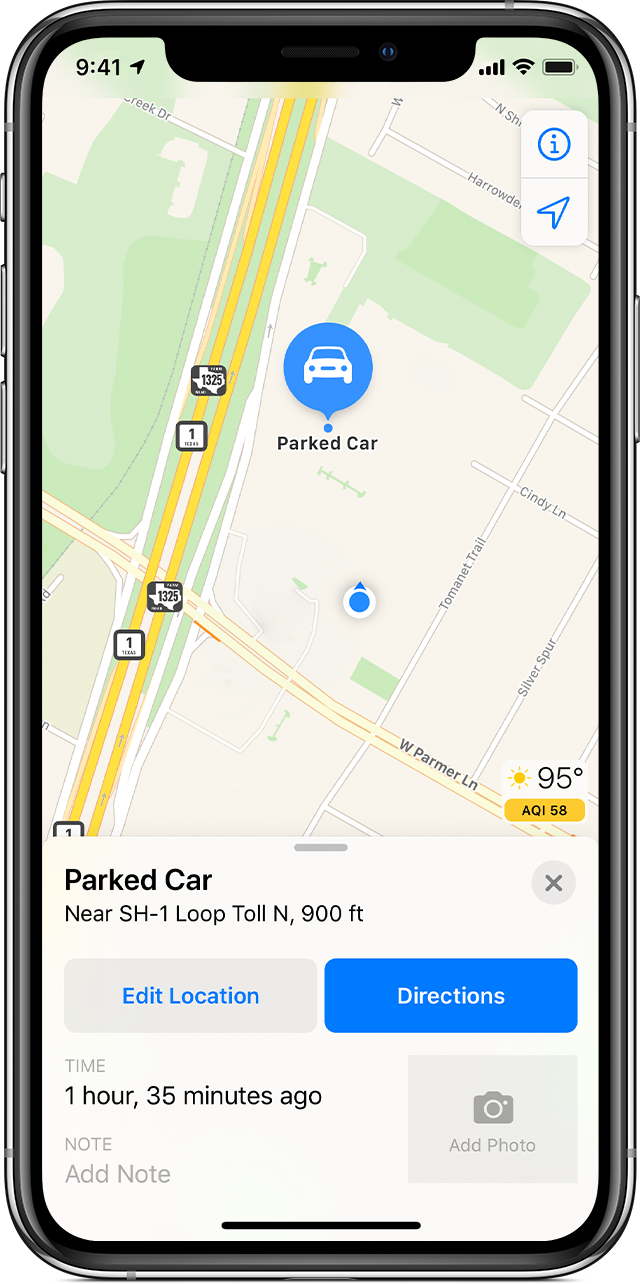
\includegraphics[width=0.3\textwidth]{images/ios13-iphone-xs-maps-parked-car.png}
  \caption{Apple Maps Parked Car, Image from Apple Support page \url{https://support.apple.com/en-us/HT207227} (last accessed October 15, 2019)}
  \label{fig:ios_park_det}
\end{figure}

Apple Maps\footnote{Apple Maps, \url{https://www.apple.com/ios/maps/}, ( last accessed  August 19, 2019}, which is preinstalled on iOS devices, supports determining the parking position of a car on an iPhone.  The parking position is determined via the phones connection to the car. When the Bluetooth connection or the CarPlay\footnote{CarPlay: \url{https://www.apple.com/ios/carplay/} (last accessed October 15, 2019)} connection, a proprietary way to connect some cars with an iPhone, is interrupted, the phone logs the current position as the parking position of the car. The user can then manually change and optimise the logged position and add a photo to the saved location to make the car even easier to find. This can be seen in Figure \ref{fig:ios_park_det}. The approach used by Apple Maps is useful for users which connect their phone to their car regularly. It is not useful for users which either do not or cannot connect their phone to their car as there is no alternative solution for these users in Apple Maps. \cite{apple:maps:parkedcar}

Google Maps\footnote{Google Maps, \url{https://apps.apple.com/us/app/google-maps-transit-food/id585027354}, (last accessed August 19, 2019)} also offers a feature to determine the parking position of a users car on an iPhone. Three different approaches are implemented. First,  the application can determine the parking position automatically via the Motion and Fitness Activity data of the user. How exactly it uses the data is not mentioned. The mentioned Motion and Fitness Activity data include data from the iPhone`s accelerometer, gyroscope and magnetometer. The second approach is, like Apple Maps, based on the phones connection to the users car. The third approach is to let the user manually set the parking location. For this, the user taps their location on the map view and choose to set the current position as parking location. Also, at the end of a navigation, the user can select their current position to be saved as parking position of their car. As Google Maps does not rely solely on the direct connection of the phone to the car, it is useful to any user, independent from the users willingness or possibility to connect their phone to their car. \cite{google:maps:app:parkedcar}  \cite{apple:CoreMotion}

In the Apple AppStore\footnote{Apple AppStore, \url{https://www.apple.com/ios/app-store/}, (last accessed August 19, 2019)} are several applications which are dedicated for finding the parked car of the user. Most of them, such as Find my Parked Car\footnote{Find my Parked Car, \url{https://apps.apple.com/us/app/find-my-parked-car/id987712319}, (last accessed August 19, 2019)}, Find My Car - Car Locator\footnote{Find My Car - Car Locator, \url{https://apps.apple.com/us/app/find-my-car-car-locator/id1295565906}, (last accessed August 19, 2019)} or Find My Car - GPS Auto Parking Reminder \& Tracker\footnote{Find My Car - GPS Auto Parking Reminder \& Tracker, \url{https://apps.apple.com/us/app/find-my-car-gps-auto-parking-reminder-tracker/id815542507}, (last accessed August 19, 2019)} approach the determination of the users car by relying on input by the user. Some applications, such as ParKing P\footnote{ParKing P, \url{https://apps.apple.com/us/app/parking-p-find-my-parked-car/id1233326914?l=en}, (last accessed August 19, 2019)}, also offer an approach based on the Bluetooth connection of the phone to the car. 

Several applications from a variety of developers exist to support users in finding their parked car. The most used navigation systems on iOS, Google Maps and Apple Maps, have this functionality build in. For determining the parking position, most apps rely on either direct user input or on a connection of the phone to the car. Only Google Maps uses some kind of movement data, the Motion and Fitness Activity data, to determine the parking position of a car. In the research, no application is found, that determines the parking position of a car based on the spatial trajectory of a user.


\section{Related Works}
The fourth section, \textit{Related Works}, discusses academic works related to the Bachelor thesis. The focus is on transportation mode classification based on spatial trajectories, as it is the base of the parking position determination approach of the thesis. No academic work related to the determination of the parking position of a car based on spatial trajectories is discussed as no academic work which covers this subject is found during the research.

\cite{Zheng:2015:TDM:2764959.2743025} is a survey on the field of trajectory data mining. It presents a categorisation of trajectory data mining, explains each category briefly and lists existing research of each category.\newline
The paper explains the high level concepts of trajectory data mining, including stay-point detection, trajectory segmentation and trajectory classification, which are used in the thesis to classify the transportation mode of a users spatial trajectories. It is also referred to as a source for several definitions, such as spatial trajectory, trajectory segmentation, and segments.

\cite{Prelipcean2017} is a survey of approaches for transportation mode detection. It introduces a classification of the approaches into three classes and lists some of the most influential academic works for each class. The first class, Location-based Services (LBS), focuses on real time classification of a transportation mode and is mostly used for systems which provides direct feedback to the users. The second class, Transportation Science (TSc), focuses on travel patterns of one or more individuals. Thus, the data does not need to be processed in real time and can take more context into account. The third class, Human Geography (HG), focuses on enriching trajectories with more semantics meaning, such as the information if a boat is fishing.\newline
The approach to determine the parking position of a car based on trajectory segmentation in the Bachelor thesis is to categorise as LBS and HG, as it aims to provide the parking position of a car, which is additional semantic meaning, in near real time when the user request the position of their parked car. 

\cite{Zheng2008} presents an approach to infer the transportation mode only from GPS trajectories. For this, the authors first segment a spatial trajectory into trips. Next, the individual trips are segmented into walk Segments and non-walk segments based on their average speed. The non-walk segments are then classified into different transportation methods: car, bus, and bike. In the last step, the probabilities of the transportation methods are adjusted based on the transportation mode of the previous segment. \newline
The Bachelor thesis relies for the determination of the parking position of a car on the transportation mode classification of the users spatial trajectory. This paper is one of the first academic work about the transport mode classification based on the spatial trajectories of a user and thus build the base of most further research in this domain.

\cite{zheng2008understanding} is a direct continuation of the authors`s previous work \cite{Zheng2008}. It improves the features and the post-processing process. The newly introduced features are heading change rate, velocity change rate and stop rate. The improved post-processing process segments the likelihood for a transportation mode into three categories and optimises the results based on the assigned category. \newline
The newly introduced features are not applicable to the chosen approach in the Bachelor thesis, as they assume a pre-segmentation into stages, before the stages are classified.

\cite{Xiao2017} classifies the transportation mode of a spatial trajectory based on tree-based ensemble methods. It does not rely on a pre-segmentation into walk and non-walk segments. The used tree ensemble based machine learning models, such as Random Forest, Gradient Boosting Decision Tree, and XGBoost show better performance than the best models of previous work, such as in \cite{Zheng2008}. The authors present 111 different features to extract from trajectory segments and reach a maximum recall of over 90\%. A limitation of the paper is the missing approach to segment unlabelled trajectories into stages which then can be classified. The paper assumes the data to be available in pre-segmented stages.\newline
The paper can be understood as a continuation of the work described in \cite{Zheng2008} with more modern machine learning models and more exhaustive features. The Bachelor thesis uses the machine learning model XGBoost, which has the best performance reported in the paper and also adapts the most important features shown in the paper, which are applicable to the used approach. \cite{chen2016xgboost}

In \cite{Bolbol2012} the transportation mode of spatial trajectories is classified by using a floating window approach. The transportation mode of fixed size floating window sets of consecutive segments is classified. Based on these classifications, stages are defined. Only speed and acceleration are used as features as they are the most discriminatory. The paper introduces the idea of sparse datasets to reduce computation costs and to save battery power on the trajectory generating device. It is concluded that 30 to 60 second intervals seem to be sufficient.\newline
The paper is highly influential to the Bachelor thesis. The floating window approach is used to avoid relying on heuristics to segment trips into segments of the same transportation mode.

\cite{lee2008traclass} presents a framework to generate features for the classification of spatial trajectories. The frameworks distinguishes between region-based and trajectory-based features.  \newline
The results of this paper are only partly adaptable for the Bachelor thesis, as the trajectory classification in the thesis solely focuses on trajectory-based features. Region-based features are avoided to ensure the independence of the transportation mode classification from the location where the spatial trajectories are generated.

\cite{zheng2010geolife} presents the social networking service ''GeoLife'' by Microsoft Asia. The goal of the project is to improve understanding of trajectories, users and locations. One of the aspects of the trajectory understanding is the transportation mode classification. In the project, spatial trajectories of several people over a long period of time are generated.\newline
The data from this project is used in the Bachelor thesis to train the machine learning model, that classifies the transportation mode of a users trajectory segments.

The dataset \cite{zheng2010geolife} \cite{zheng2008understanding} \cite{geolife-dataset} \cite{zheng2009mining} contains GPS trajectories collected for the GeoLife project from Microsoft Research Asia. 91 \% of the reported trajectories consist of relatively dense points, which are reported every 2-5 seconds or 5-10 meters. The data is created by 182 users over three years. 69 of the users labeled their trajectories with the used transportation mode. \newline
The dataset is used to train a machine learning model, which classifies the transportation modes of a users trajectory. Based on the change points and the transportation modes of the adjacent trip segments, the parking position of the drivers car is determined. 

\cite{Dabiri2018} discusses a convolutional neural network approach to classify the transportation mode of spatial trajectories. It is argued that this approach avoids the manual creation of high level features which are error prone and nor exhaustive. They reach an accuracy of 84.8\%.\newline
The paper describes in detail the pre-processing steps of the training data for the machine learning model. They introduce a limit for the average acceleration and speed of a stage for each transportation mode to filter wrongly labeled data. The used values are the basis of a pre-processing step in the Bachelor thesis.

The presented papers give an overview of the research in the field of transport mode classification of spatial trajectories. Earlier papers rely on relatively simple machine learning approaches, such as Decision Trees, while recent papers use more complex systems, such as XGBoost or convolutional neural networks. Most research reaches an accuracy between 80\% and 95\%. \cite{Zheng2008} \cite{Xiao2017} \cite{Dabiri2018}